\section{Code Generation}

Having completed semantic analysis, the compiler
can proceed to code generation.

\subsection{Passing on the Environment Tree}

Before, proceeding onto to the details of code generation it is
important to note that here is were all the upfront work that
was put into making Environment trees, the data structure of
choice for managing scopes, pays off. This is because there is
no need to re-stablish the types of any of the variables, at any
scope in a program.

\begin{lstlisting}[caption={Getting the global environment from
the \texttt{AnalysisVisitor} and passing it on for reordering
and code generation (runner/Runner.cpp)}]
    std::unique_ptr<Environment> environment =
        mAnalyser.getEnvironment();

    ReorderVisitor reorder{};

    reorder.reorderAst(ast.get());

    if (mParserDbg) {
        debugParsing(ast.get());
    }

    reorder.reorderEnvironment(environment.get());

    GenVisitor gen{environment.get()};
\end{lstlisting}

\subsubsection{The \texttt{TypeVisitor} Class}

Having said that there is still the need to recompute the types
of expressions since the type of a composite expression e.g.
\texttt{2 + 3} cannot be stored in an Environment. To handle
this another visitor, this time called \texttt{TypeVisitor} was
created.

\begin{todo}
In the event that type checking/generation is completely
delegated to the \texttt{TypeVisitor} future version of compiler
can drop usage of Environment trees in favour of re-computing
types as requested. Additionally, such a change improves memory
usage in exchange for time as described in
\ref{sss:memoryadvantage}.
\end{todo}

\begin{lstlisting}[caption={The \texttt{visit(FunctionCall *)}
method in the \texttt{TypeVisitor} class
(ir\_gen/TypeVisitor.cpp)}, label=lst:recomputefunctype]
void TypeVisitor::visit(core::FunctionCall *expr) {
    std::optional<Symbol> symbol{
        findSymbol(expr->identifier, mRefStack.getGlobal())
    };

    mReturn = symbol->as<FunctionSymbol>().returnType;

    expr->core::Expr::accept(this);
}
\end{lstlisting}

Currently, a \texttt{TypeVisitor} is given a \texttt{RefStack}
for environment access and its main capability is re-calculating
the type of \textbf{already} type-checked expressions, see
\listref{recomputefunctype}.

\begin{marker}
Usage of a \texttt{TypeVisitor} on a non-type-checked expression
will at best crash and at worst, still work, leading to
undefined behaviour.
\end{marker}

\subsection{Reordering}\label{sss:reordersec}

Due to the fact that the \texttt{PArDis} VM Simulator expects
all functions to be defined before the \texttt{.main} segment,
which in the case of \texttt{PArL} is everything not in a
function declaration, a solution needs to be devised to ensure
that this order requirement is satisfied.

A solution to this problem can be achieved by reordering the AST
and Environments. This is because function declarations can only
exist in global scope, and hence moving them such that they are
the first statements, which are encountered in a program is a
sufficient constraint to ensure code generation as required by
the VM.

\begin{todo}
Currently the compiler has support for named scopes (see
backend/Environemnt.cpp, lines 25 and 34). With a specially
designed naming scheme to uniquely identify each scope, support
for nested functions can be enable by mangling function names
with scope names and lifting function declarations into global
scope.
\end{todo}

This approach required two visitors, named
\texttt{IsFunctionVisitor} and \texttt{ReorderVisitor}, and a
function \texttt{reorderEnvironment()} (the choice to embed it
into the \texttt{ReorderVisitor} was arbitrary).

The \texttt{IsFunctionVisitor} is quite self-explanatory it is a
very simple visitor with an exposed method \texttt{check()}
which returns true only if a node is a function declaration.

\begin{lstlisting}[caption={The \texttt{reorder()} method in the
\texttt{ReorderVisitor} class (preprocess/ReorderVisitor.cpp)}]
void ReorderVisitor::reorder(
    std::vector<std::unique_ptr<core::Stmt>> &stmts
) {
    for (auto &stmt : stmts) {
        if (isFunction.check(stmt.get())) {
            mFuncQueue.push_back(std::move(stmt));
        } else {
            mStmtQueue.push_back(std::move(stmt));
        }
    }

    stmts.clear();

    for (auto &stmt : mFuncQueue) {
        stmts.push_back(std::move(stmt));
    }

    for (auto &stmt : mStmtQueue) {
        stmts.push_back(std::move(stmt));
    }

    reset();
}
\end{lstlisting}

The \texttt{ReorderVisitor} implements a single method
\texttt{reorder()} which is called only for program and block
nodes. The \texttt{reorder()} makes use of two queues. The first
queue keeps track of function declarations and the second queue
keeps track of everything else. The \texttt{reorder()} method
traverse the provided statement vector and enqueues statements
in there respective queues. Then the elements of the first queue
are dequeued back into the vector and then the elements of the
second queue are dequeued back into the vector. Due to the usage
of queues this essentially moves all function declarations in
their original order as the first elements of the statements
vector. The visitor is then accepted by all the reordered
statements.

\begin{note}
The visitor is accepted by the reordered statements, to cater
for the case when function declarations are also present in
other scopes not just the global scope. However, this is
currently not the case (see analysis/AnalysisVisitor.cpp, line
955).
\end{note}

\subsection{Function Declarations}

Due to the reordering described in \ref{sss:reordersec}, the
first nodes to be emitted are function declarations.

\begin{lstlisting}[escapechar=!, caption={The
\texttt{visit(FunctionDecl *)} method in the \texttt{GenVisitor}
class (ir\_gen/GenVisitor.cpp)}, label=lst:genfuncdecl]
void GenVisitor::visit(core::FunctionDecl *stmt) {
    Environment *nextEnv = mRefStack.peekNextEnv();

    size_t aritySize{0};

    for (auto &stmt : stmt->params) {
        aritySize +=
            !\colorbox{UMPaleRed}{mDeclCounter.count(stmt.get(),\
            nextEnv);}!
    }

    !\colorbox{UMPaleRed}{emit_line(".\{\}",\
    stmt->identifier);}!

    mRefStack.pushEnv(aritySize);

    for (auto &param : stmt->params) {
        !\colorbox{UMPaleRed}{param->accept(this);}!
    }

    stmt->block->accept(this);

    mRefStack.popEnv();
}
\end{lstlisting}

Again for code generation two more visitors apart from the
\texttt{TypeVisitor} were used. These are the
\texttt{GenVisitor} and the \texttt{VarDeclCountVisitor}.

\begin{lstlisting}[caption={The \texttt{visit(VariableDecl *)}
method in the \texttt{VarDeclCountVisitor} class
(ir\_gen/VarDeclCountVisitor.cpp)}, label=lst:vardeclcount]
void VarDeclCountVisitor::visit(core::VariableDecl *stmt) {
    std::optional<Symbol> symbol =
        mEnv->findSymbol(stmt->identifier);

    auto &variable = symbol->asRef<VariableSymbol>();

    mCount += variable.type.is<core::Array>()
                  ? variable.type.as<core::Array>().size
                  : 1;
}
\end{lstlisting}

The \texttt{GenVisitor} as its name suggest is the main visitor
which produces the VM instructions. The
\texttt{VarDeclCountVisitor} is an additional visitor which is
used to calculate the size of the memory required when opening a
frame on the VM.

\begin{note}
Within the VM memory is implemented in the form a JavaScript
array. This means that there are no restrictions on how big a
single location is. For this reason there is not true standard
unit of size. However, it is implicitly assumed that the base
types: \texttt{bool}, \texttt{int}, \texttt{float} and
\texttt{color} all occupy single unit. Hence, when calculating
the size of for example \texttt{int[4]} the
\texttt{VarDeclCountVisitor} returns $4$ (see
\listref{vardeclcount}).
\end{note}

\begin{lstlisting}[caption={The \texttt{emit\_line()} method in
the \texttt{GenVisitor} class (ir\_gen/GenVisitor.cpp)},
label=lst:emitline]
template <typename... T>
void emit_line(fmt::format_string<T...> fmt, T &&...args) {
    mCode.push_back(fmt::format(fmt, args...));
}
\end{lstlisting}

On the other hand, the main mechanism with which the
\texttt{GenVisitor} emits VM code is \texttt{emit\_line()}.
Again similar to \texttt{error()} and \texttt{warning()} from
other visitors, \texttt{emit\_line()} wraps an \texttt{fmtlib}
function to allow for a nicer overall developer experience when
formatting strings, see \listref{genfuncdecl}.

In the context of function declarations the only significant
usage of \texttt{emit\_line()} is to output the identifier of
the function.


\begin{lstlisting}[caption={The \texttt{visit(FormalParam *)}
method in the \texttt{GenVisitor} class
(ir\_gen/GenVisitor.cpp)}, label=lst:formalparam]
void GenVisitor::visit(core::FormalParam *param) {
    Environment *env = mRefStack.currentEnv();

    std::optional<Symbol> symbol =
        env->findSymbol(param->identifier);

    core::abort_if(
        !symbol.has_value(),
        "symbol is undefined"
    );

    size_t idx = env->getIdx();

    auto variable = symbol->as<VariableSymbol>();

    if (variable.type.is<core::Base>()) {
        env->incIdx();
    } else if (variable.type.is<core::Array>()) {
        env->incIdx(variable.type.as<core::Array>().size);
    } else {
        core::abort("unknown type");
    }

    // NOTE: make sure this is actually a reference.
    env->getSymbolAsRef(param->identifier)
        .asRef<VariableSymbol>()
        .idx = idx;
}
\end{lstlisting}

Next, specific attention has to be given to the formal
parameters of a function declaration (what will be discussed
also applies to normal variable declarations within a scope).
Referencing of formal parameters or variables within the VM is
done with the instruction \mbox{\texttt{push [i:l]}} (for
behaviour see \figref{framesexp}). The key take-away from how
this instruction works is the fact that frames (which are
actually just memory) are accessed via an index (in the
instruction \texttt{i}).

Hence, during code generation any reference to a formal
parameter or variable needs to happen through an index. This is
why, when defining a new formal parameter or variable, the
internal index of the current environment is copied into the
formal parameter or variable's associated symbol. This
facilitates referencing a formal parameter or variable in the VM
code (see \listref{formalparam} and ir\_gen/GenVisitor.cpp, line
105).

Additionally, the index of the environment is incremented to the
next free position i.e. the next position a new formal parameter
or variable can be stored within the frame.

\begin{figure}[H]
\centering
\begin{mdframed}[backgroundcolor=UMPaleRed]
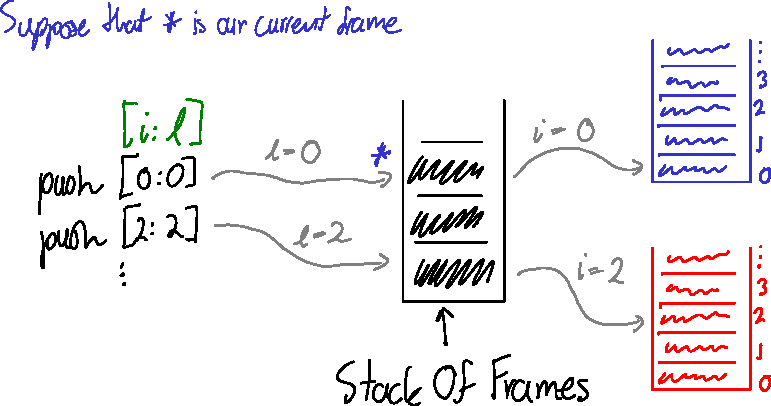
\includegraphics[width=\linewidth]{framesexp.pdf}
\end{mdframed}
\caption{A pictorial example of how the \mbox{\texttt{push
[i:l]}} operates}
\label{fig:framesexp}
\end{figure}

\subsubsection{Properly Closing Scopes}

A very important consideration when it comes to
function declarations is closing of scopes.

This is a problem of interest because functions should be
capable of returning anywhere within the body of a function even
if they are nested within multiple scopes.

\subsection{Scopes \& Variable Declarations}

\subsection{Expressions}

\subsubsection{Type Specific VM Code}

\subsubsection{Accessing Variables}

\subsubsection{Function Calls}

\subsection{Branching}
